% Titelseite:

\title{
  \textbf{Sch�tzung und Kalibrierung von Copulae}\\
  ~~\\
    \emph{Welche Copula passt zu meinen Daten?} \\
  Implementierung von Sch�tzungsmethoden f\"ur den bivariaten Fall in
  \emph{R}
  \\~\\
  \begin{figure}[h]  
  	\centering
    \begin{minipage}[b]{.3\textwidth} % [b] => Ausrichtung an \caption
      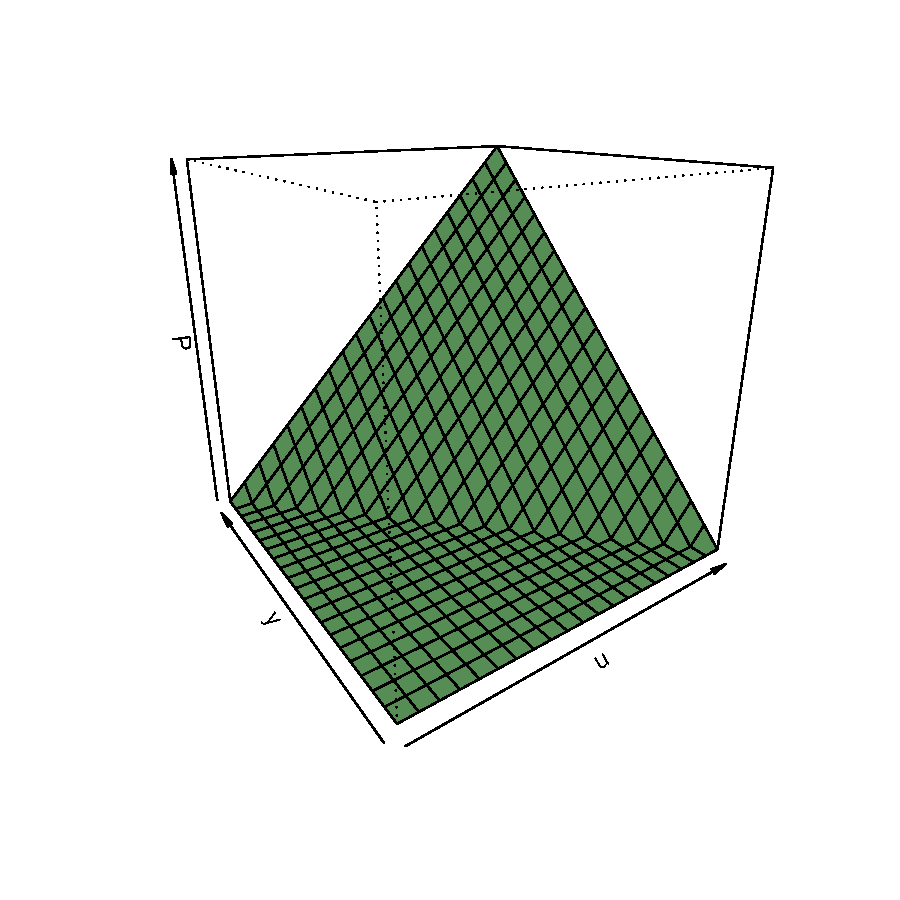
\includegraphics[width = \textwidth]{copulaM.pdf}
    \end{minipage}
    \hspace{.0\linewidth}% Abstand zwischen Bilder
    \begin{minipage}[b]{.3\textwidth} % [b] => Ausrichtung an \caption
      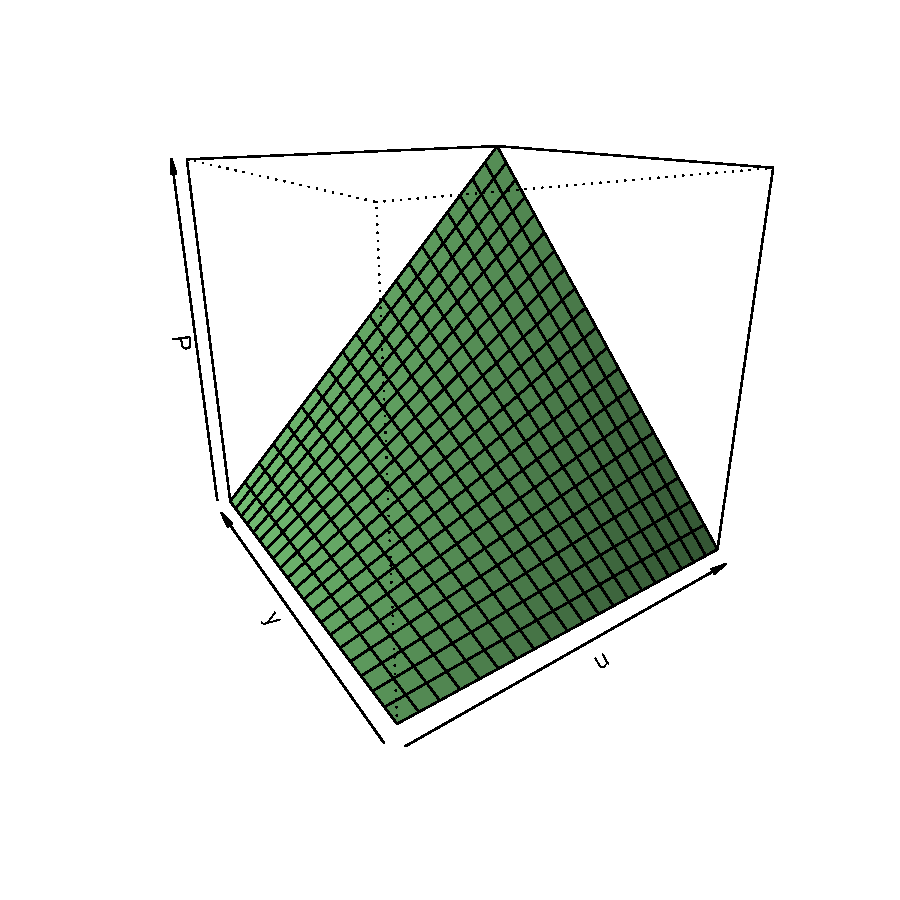
\includegraphics[width = \textwidth]{copulaPi.pdf}
    \end{minipage}
    \hspace{.0\linewidth}% Abstand zwischen Bilder
    \begin{minipage}[b]{.3\textwidth} % [b] => Ausrichtung an \caption
      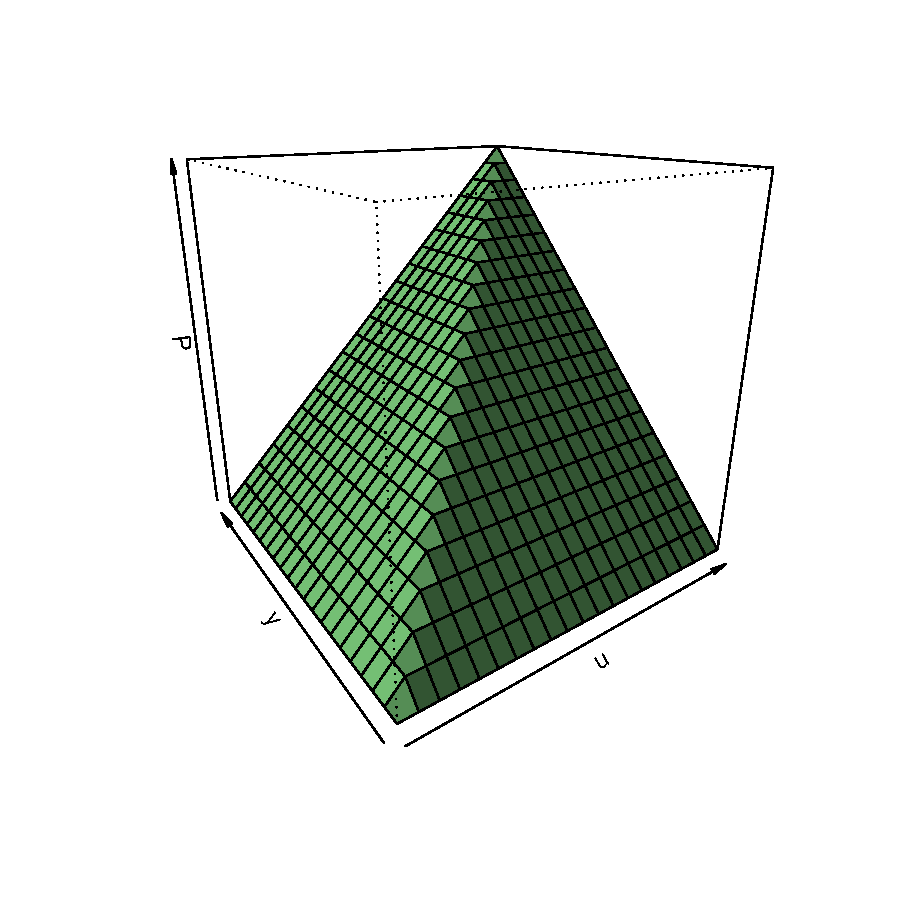
\includegraphics[width = \textwidth]{copulaW.pdf}
    \end{minipage}
  \end{figure}
}

\author{
  Gerold K�b (0250001)\\
  Martin Gartner (0351427)
}